%\documentclass{acm_proc_article-sp}

%\documentclass{article}

\documentclass{llncs}

\usepackage{wrapfig}
\usepackage{mathpartir}
\usepackage{turnstile}
\usepackage{amssymb}
\usepackage{amsmath}
\usepackage{stmaryrd}
\usepackage{graphicx}
\usepackage{epsfig}
\usepackage{subfigure}
\usepackage{listings}
\usepackage{natbib}
\usepackage{verbatim}
\usepackage[utf8]{inputenc}
\usepackage[T1]{fontenc} 
\usepackage[hyphens]{url}
\lstset{language=ml}
\lstset{commentstyle=\textit}
\lstset{mathescape=true}
\lstset{backgroundcolor=,rulecolor=}
\lstset{frame=single}
\lstset{breaklines=true}
\lstset{basicstyle=\scriptsize\ttfamily}

\DeclareMathOperator{\wf}{wf}
\DeclareMathOperator{\acyclic}{acyclic}
\DeclareMathOperator{\Linear}{Linear}
\DeclareMathOperator{\NonLinear}{NonLinear}
\DeclareMathOperator{\range}{range}
\DeclareMathOperator{\FV}{FV}
\DeclareMathOperator{\LFV}{LFV}
\DeclareMathOperator{\rule-fun}{rule-fun}

\begin{document}

\title{Designing Casanova: a language for games}

\author{
G. Maggiore, \ A. Span\`o, \ R. Orsini, \ G. Costantini, \ M. Bugliesi, \ M. Abbadi \\[1mm]
}

\institute{Universit\`a Ca' Foscari Venezia \\[1mm]
DAIS - Computer Science \\[1mm]
\email{\{maggiore,spano,orsini,costantini,bugliesi,mabbadi\}@dais.unive.it}
}       

\date{}

\maketitle

\begin{abstract}
Games are extremely complex pieces of software which give life to animated virtual worlds. Game developers carefully search the difficult balance between quality and efficiency in their games.

In this paper we present the Casanova language. This language allows the building of games with three important advantages when compared to traditional approaches: simplicity, safety and performance. We will show how to rewrite an official sample of the XNA framework, resulting in a smaller source and higher performance.
\end{abstract}

\begin{comment}
\category{D.1.1}{Programming Techniques}{Applicative (Functional) Programming} 
\category{D.2.2}{Soft\-ware Engineering}{Software Libraries}[Design Tools and Techniques]
\category{D.2.13}{Soft\-ware Engineering}{Reusable Software}[Domain engineering, Reusable libraries, Reuse models]
\category{D.3.3}{Programming Languages}{Language Constructs and Features}
\category{D.3.4}{Pro\-gramming Languages}{Processors}[Optimization, Run-time environments]
\category{H.5.1}{Information Systems}{Information Interfaces and Presentation}[Multimedia Information Systems]

\terms{Games,Performance,Languages}

\keywords{games, optimization}
\end{comment}

\section{Introduction}
\label{sec:introduction}
%%%%%%%%%%%%%%%%%%%%%%%%%%%%%%%%%%%%%%%%%%%%%%%%%%%%%%%%%%
% intro.tex
%%%%%%%%%%%%%%%%%%%%%%%%%%%%%%%%%%%%%%%%%%%%%%%%%%%%%%%%%%

%%%%%%%%%%%%%%%%%%%%%%%%%%%%%%%%
%edit
%%%%%%%%%%%%%%%%%%%%%%%%%%%%%%%%
Computer games promise to be the next frontier in entertainment, with game sales being comparable to movie and music sales in 2010 \cite{ESA}. 

This unprecedented market prospects and potential for computer-game diffusion among end-users has created substantial interest in research on principled design techniques and on cost-effective development technologies for game architectures. Our present endeavour makes a step along these directions. 

Making games is an extremely complex business. Games are large pieces of software with many heterogeneous requirements, the two crucial being high quality and high performance \cite{GAME_OPT}. 


%%%%%%%%%%%%%%%%%%%%%%%%%%%%%%%%
%edit
%%%%%%%%%%%%%%%%%%%%%%%%%%%%%%%%
High-quality in games is comprised by two main factors: visual quality and simulation quality. Visual quality in games has made huge leaps forward, and many researchers continuously push the boundaries of real-time rendering towards photorealism. Simulation quality, on the other hand, is often lacking in modern games; game entities often react to the player with little intelligence, input controllers are used in simplistic ways and the logic of game levels is more often than not completely linear. Building a high-quality simulation is very complex in terms of development effort and also results in computationally expensive code. To make matters worse, gameplay and many other aspects of the game are modified (and often even rebuilt from scratch) many times during the course of development. For this reason game architectures require a lot of flexibility.

To manage all this complexity, game developers use a variety of strategies. Object-oriented architectures, components, reactive progamming, etc have all been used with some degree of success for this purpose \cite{COMPONENTS1,GAMEOBJECTS,FRP}. 

In this paper we will present the Casanova language, a language for making games. Casanova offers a mixed declarative/procedural style of programming which has been designed in order to facilitate game development. The basic idea of the language is to require from the developer only and exclusively those aspects of the game code which are specific to the game being developed. The language aims for simplicity and expressive power, and thanks to automated optimizations it is capable of generating code that is much faster than hand-written code and at no effort for the developer. The language offers primitives to cover the development of the game logic, and incorporates the typical processing of a game engine. Also, the language is built around a theoretical model of games with a ``well-formedness'' definition, in order to ensure that game code is always a good model of the simulated virtual world.

In the remainder of the paper we show the Casanova language in action. We begin with a description of the current state of game engines and game programming in Section \ref{sec:background}. In Section \ref{sec:model} we define our model of games. We describe the Casanova language in Section \ref{sec:casanova}.  We show an example of Casanova in action, and also how we have rewritten the game logic of an official XNA sample from Microsoft \cite{XNA_SAMPLES} in Casanova with far less code and higher runtime performance in Section \ref{sec:case_study}. In Section \ref{sec:conclusions} we discuss our results and some future work.
 

\section{Background}
\label{sec:background}
%%%%%%%%%%%%%%%%%%%%%%%%%%%%%%%%%%%%%%%%%%%%%%%%%%%%%%%%%%
% background.tex
%%%%%%%%%%%%%%%%%%%%%%%%%%%%%%%%%%%%%%%%%%%%%%%%%%%%%%%%%%

In this section we discuss some current approaches to game development.

The two most common game engine architectures found in today's commercial games are object-oriented hierarchies and component-based systems.

In a traditional object-oriented game engine the hierarchy represents the various game objects, all derived from the general \texttt{Entity} class. Each entity is responsible for updating itself at each tick of the game engine \cite{OO_GAME_DEV}.

A component-based system defines each game entity as a composition of components that provide reusable, specific functionality such as animation, movement, reaction to physics, etc. Component-based systems are being widely adopted, and they are described in \cite{COMPONENTS1}.

These two, more traditional approaches both suffer from a noticeable shortcoming: they focus exclusively on representing single entities and their update operations in a dynamic, even composable way. By doing so they lose the focus on the fact that most entities in a game need to \textit{interact} with one another (collision detection, AI, etc.), and usually lots of a game complexity comes from defining (and optimizing) these interactions. Also, all games feature behaviors that take longer than a single tick; these behaviors are hard to express inside the various entities, which often end up storing explicit program counters to resume the current behavior at each tick.

There are two more approaches that have emerged in the last few years as possible alternatives to object-orientation: (functional) reactive programming and SQL-style declarative programming.

Functional reactive programming (FRP, see \cite{FRP}) is often studied in the context of functional languages. FRP programming is a data-flow approach where value modification is automatically propagated along a dependency graph that represents the computation. FRP offers a solution to the problem of representing long-running behaviors, even though it does not address the problem of many entities that interact with each other.

SQL-queries for games have been used with a certain success in the SGL language (see \cite{SCALING_GAMES}). This approach uses a lightweight, statically compiled query engine for defining a game. This query engine is aggressively optimized, in order to make it simple to express efficient aggregations and cartesian products, two very common operators in games. On the other hand, SGL suffers when it comes to representing long-running behaviors, since it focuses exclusively on defining the tick function.

We have designed Casanova with these two issues in mind: with Casanova, the integration of the interactions between entities and long-running behaviors is seamless. 

\section{A Model for Games}
\label{sec:model}
%%%%%%%%%%%%%%%%%%%%%%%%%%%%%%%%%%%%%%%%%%%%%%%%%%%%%%%%%%
% model.tex
%%%%%%%%%%%%%%%%%%%%%%%%%%%%%%%%%%%%%%%%%%%%%%%%%%%%%%%%%%

We define a game as a triplet of a game state, an update function and a series of asynchronous behaviors. In this model we purposefully ignore the drawing function, since it is not part of the current design of Casanova.

\begin{lstlisting}
type Game 's =  
  { State : 's; Update : 's -> DeltaTime -> (); Behavior : 's -> () }
\end{lstlisting}

The game state is a set of (homogeneous) collections of entities; each entity is a collection of attributes, which can either be \textit{(i)} primitive values, \textit{(ii)} collections of attributes or \textit{(iii)} references to other entities.

The update function modifies the attributes of the entire state according to a fixed scheme which does not vary with time; we call this fixed scheme the \textbf{rules} of the game; rules can be physics, timers, scores, etc. Each attribute of each entity is associated to exactly one rule. The update function is quick and must terminate after a brief computation, since it is invoked in a very tight loop that should perform 60 iterations per second.

The behavior function is a sequential process which performs a series of operations on the attributes of the game entities. It is a long-running, asynchronous process with its own local state, it runs in parallel with the main loop and it can access the current clock time at any step to perform actions which are synchronized with real time. The processing over the game state that a behavior performs usually takes more than one tick; behaviors are used, for example, for implementing AIs.

A game engine is thus a certain way of processing a game:

\begin{lstlisting}
let run_game (game:Game 's) =
  let rec run_rules (t:Time) =
    let t' = get_time()
    game.Update game.State (t'-t)
    run_rules t'
  parallel (run_rules (get_time()), game.Behavior(game.State))
\end{lstlisting}


We define four properties of a correct and well-behaved game: \textit{(i)} each entity is updated exactly once per tick, \textit{(ii)} entity update is order-independent, \textit{(iii)} tick always terminates and \textit{(iv)} the game runs at an interactive framerate.

Casanova guarantees only the first three requirements. The fourth requirement cannot be guaranteed, since it heavily depends on factors such as the size of the virtual world and the computational resources of the machine used to run the game; nevertheless, by automating certain optimizations Casanova makes it easier to achieve the fourth requirement.



%%%%%%%%%%%%%%%%%%%%%%%%%%%%%%%%
%edit
%%%%%%%%%%%%%%%%%%%%%%%%%%%%%%%%
\subsection{Architecture of a Casanova Game}

We now discuss the architecture of a Casanova game.

\begin{wrapfigure}{r}{0.4\textwidth}
\centering
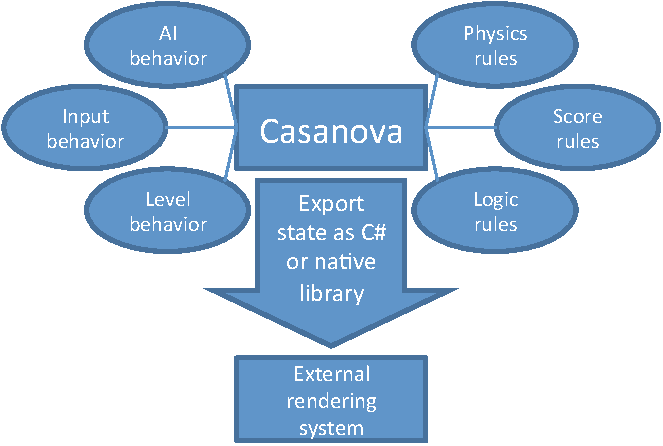
\includegraphics[width=0.5\textwidth]{architecture.pdf}
\caption{Game architecture with Casanova}
\noindent
%\hrulefill
\label{test}
\end{wrapfigure}

Behaviors are used to make it easier to build complex input, articulated level logics or customized AI algorithms into the game. While Casanova does not (yet) integrate any deduction engine or proper AI system, it makes integrating such a system with the game loop and the game state much simpler.

Rules are used to build all the regular logic that the game continuously repeats, for example the fact that when projectiles collide with an asteroid then the asteroid is damaged or other logical relationships between entities. Rules are the main workhorse of a game, and Casanova ensures that all the queries that make up the various rules maintain the integrity of the state and are automatically optimized to yield faster runtime.

The Casanova compiler will then export the game state as a series of type definitions and classes that can be accessed directly (that is without any overhead) from a C\# or C++ rendering library; this way existing rendering code and engines can be integrated with Casanova with little effort.
 

\section{The Casanova language}
\label{sec:casanova}
%%%%%%%%%%%%%%%%%%%%%%%%%%%%%%%%%%%%%%%%
% THE CASANOVA LANGUAGE
%%%%%%%%%%%%%%%%%%%%%%%%%%%%%%%%%%%%%%%%

In this section we present the Casanova language syntax, typing rules and semantics. 

\begin{center}
\line(1,0){240}
\end{center}

\textit{Note on syntactic sugar:}

We will use the following syntactic sugar to increase source code readability:

Rather than write:

\begin{lstlisting}
let! _ = b1
in b2
\end{lstlisting}

we can write:

\begin{lstlisting}
do! b1
in b2
\end{lstlisting}

Rather than write:

\begin{lstlisting}
let x = t1
in let y = t2
in t3
\end{lstlisting}

we can write:

\begin{lstlisting}
let x = t1
let y = t2
t3
\end{lstlisting}

\begin{comment}
We may also directly iterate all the elements of a table \texttt{t} by writing:

\begin{lstlisting}
for x in t do
  action
\end{lstlisting}

rather than explicitly using indices or \texttt{head} and \texttt{tail}.
\end{comment}

\begin{center}
\line(1,0){240}
\end{center}

\subsection{Simple Example}

Before we start, we will give a general idea of how the language works with a small example. We will build a very simple game where asteroids enter the screen from the top, scroll down to the bottom at different velocities and then disappear.

A Casanova program is composed of two portions:
\begin{itemize}
\item the state of the game, a series of types arranged hierarchically (typically at least one for the global state and one for the state of each entity); each portion of the game state may contain exactly one rule (a function that computes the new value of the field)
\item the main behavior, which performs a series of instructions on all the mutable fields of the state (those marked as \texttt{Rule T} or \texttt{Var T}; behavior execution is suspended at the \texttt{yield} statement, and resumed at the next tick
\end{itemize}

The state of our simple program is defined as:

\begin{lstlisting}
type Asteroid =
  {
    Y     : Rule float
          :: \(self,y,dt) -> y + dt * self.VelY
        
    VelY  : float        
    X     : float
  }

type GameState =
  {
    Asteroids           
        : Rule(Table Asteroid)
        :: \asteroids -> [a | a <- asteroids && a.Y > 0]
  	    
    DestroyedAsteroids	
        : Rule<int>
        :: \(state,destroyed_asteroids) -> destroyed_asteroids + count([a | a <- !state.Asteroids && a.Y <= 0])
  }
\end{lstlisting}
  
In a type declaration, the \texttt{:} operator means ``has type'', while the \texttt{::} operator means ``has rule''. Rules can access the game state, the current entity and the time delta between the current and previous ticks.

In the state definition above we can see that the state is comprised by a set of asteroids which are removed when they reach the bottom. Removing these asteroids increments a counter, which is essentially the ``score'' of our game. Each asteroid moves according to its velocity.

The initial state is then provided:
\begin{lstlisting}
let state0 =
  {
    Asteroids               = []
    DestroyedAsteroids      = 0
  }
\end{lstlisting}

After defining the state we must give an initial behavior. As can be easily noticed, our game does not generate any asteroids and so the initial state will never change. Since creating asteroids is an activity that certainly must not be performed at every tick (otherwise we could generate in excess of 60 asteroids per second: clearly too many), we need a function that is capable of performing \textit{different} operations on the state depending on time. Since rules perform the \textit{same} operation at every tick, they are unsuited to this kind of processing. Behaviors are built exactly around this need. The behavior for our game is the following:

\begin{lstlisting}
let main state =
  let random = mk_random()
  let rec wait interval =
    {
      let! t0 = time
      do! yield
      let! t = time
      let dt = t - t0
      if dt > interval then
        return ()
      else
        do! wait (interval - dt)
    }  
  let rec behavior() =
    {
      do! wait (random.Next(1,3))
      do! state.Asteroids.Add
      	  {
      	    X     = random.Next(-1,+1)
      	    Y     = 1
      	    VelY  = random.Next(-0.1,-0.2)
      	  }
      if state.DestroyedAsteroids < 100 then
        do! behavior()
      else
        return ()
    }
  in behavior()
\end{lstlisting}
  
Our behavior declares a random number generator and then starts iterating a function that waits between 1 and 3 seconds and then creates a random asteroid. When the number of destroyed asteroids is greater than 100, the function stops and the game ends (games end when their main behavior terminates).

Notice that behaviors are expressed with two different syntaxes: an ML-style syntax for pure terms (those which read the state and simply perform computations) and an imperative-style syntax for impure terms (those which write the state and interact with time such as wait). The imperative syntax loosely follows the monadic syntax of the F\# language, where a monadic block is declared within \texttt{\{\}} parentheses, monadic operations are preceded by either \texttt{do!} or \texttt{let!} and returning a result is done with the \texttt{return} statement.

\subsection{Syntax}
In the remainder of this section we will adopt the following conventions:
\begin{itemize}
\item capitalized items such as \texttt{Program} and \texttt{StateDef} are grammatical elements
\item quoted items such as \texttt{`type'} and \texttt{`GameState'} are keywords that must appear as indicated
\item items surrounded by \texttt{[ ]} parentheses such as \texttt{[EntityName]} are user-defined strings
\end{itemize}

The program syntax starts with the definition of the state (a series of type definitions with rules) and is followed by the entry point (the initial state and the initial behavior):

\begin{lstlisting}
Program  ::= StateDef
             Main
StateDef ::= EntityDefs
\end{lstlisting}

A type definition is comprised of one of various primitive types such as integers, floating point numbers, two- or three- dimensional vectors, etc. combined into any of the usual composite types known to functional programmers such as tuples, functions, records and sum types. Also, type declarations may contain a rule (which is simply a term, even though with the limitation that only pure functional terms are allowed inside rules). Finally, there are two types for describing behaviors; \texttt{UnsafeBehavior T} which represents an unsafe behavior which may never \texttt{yield}, and \texttt{SafeBehavior T} which represents a safe behavior which never loops indefinitely without \texttt{yield}-ing.

\begin{lstlisting}
TypeDef  ::= TypeDef'
           | TypeDef' :: Rule
          
TypeDef' ::= `()' | `int' | `float' | `Vector2' | ...
           | TypeDef $\times$ TypeDef
           | TypeDef $\rightarrow$ TypeDef
           | `{' Labels `}'
           | TypeDef $+$ TypeDef
           | Modifier TypeDef
           | `UnsafeBehavior' TypeDef
           | `SafeBehavior' TypeDef
           | [EntityName]
           
Labels   ::= Label; Labels
           | Label
           
Label    ::= [Name] `:' TypeDef
                     
Rule     ::= Term
\end{lstlisting}

A \texttt{Modifier} for a type definition allows to make a field mutable (\texttt{Rule} or \texttt{Var}), or to use queries to manipulate that field (\texttt{Table}). Also, another important modifier is \texttt{Ref} which can be seen as a programmer annotation that tells the compiler how a certain field is just a pointer to another portion of the state and as such it must not be processed recursively:

\begin{lstlisting}
Modifier  ::= Rule
            | Var
            | Table
            | Ref
\end{lstlisting}

Entities are definied as a series of type definitions with a name which can be referenced anywhere in the state; the last entity to be defined is the game state itself:

\begin{lstlisting}
EntityDefs  ::= `type' `GameState' = TypeDef
              | EntityDef
                EntityDefs

EntityDef   ::= `type' [EntityName] `=' TypeDef
\end{lstlisting}

The various entity names are simply replaced with their type definition in the remainder of the program, according to the $\llbracket \bullet \rrbracket_{\mathtt{MAIN}}$ translation rule:

\begin{mathpar}
\llbracket \mathtt{type\ EntityName\ =\ TypeDef;\ EntityDefs; Main} \rrbracket_{\mathtt{MAIN}} = 
\llbracket \mathtt{EntityDefs; \ Main} \rrbracket_{\mathtt{MAIN}} \mathtt{[EntityName} \mapsto \mathtt{TypeDef]}

\and 

\llbracket \mathtt{TypeDef;\ Main} \rrbracket_{\mathtt{MAIN}} = \mathtt{TypeDef;\ Main}
\end{mathpar}

The actual type definition of the state may be extracted from the program with the $\sigma(\bullet)$ function, which extracts the type definition and erases all the rules from it; this means that two entities may have the same type with different sets of rules. The function inductively removes all rules from a type declaration:

\begin{mathpar}
\sigma(\mathtt{Entity; EntityDefinitions}) = \sigma(\mathtt{EntityDefinitions})
\and 

\sigma(\mathtt{`type GameState = ' TypeDefinition}) = \sigma(\mathtt{TypeDefinition})
\and 

\sigma(\mathtt{T :: rule}) = \sigma(T)
\and 

\sigma(\mathtt{T}_1 \stackrel{\times}{\stackrel{+}{\mathtt{...}}} \mathtt{T}_2) = 
  \sigma(\mathtt{T}_1) \stackrel{\times}{\stackrel{+}{\mathtt{...}}} \sigma(\mathtt{T}_2)
\and 


\and 

\\ (...) \\
\end{mathpar}

A term can be a simple, ML-style functional term (we do not give all these possible definitions because they are fairly known) or an imperative behavior. Functional terms can read variables with the \texttt{!} operator and can use a Haskell-style table-comprehension syntax:

\begin{lstlisting}
Term        ::= `let' [Var] `=' Term 
                `in' Term
              | `letrec' [Var] `=' Term 
                `in' Term
              | `if' Term `then' 
                   Term 
                `else' 
                   Term
              | Term Term
              | !Term
              | `add' Term Term
              | ... (* other ML-style terms: fun, types, head, tail for tables, etc. *)
              | [ Term | Predicates ]
              | `{' Behavior `}'
              
Predicates  ::= $\epsilon$
              | [Var] `<-' Term, Predicates
              | Term, Predicates
\end{lstlisting}

A behavior defines an imperative coroutine that is capable of reading and writing the state and manipulating time. Behaviors can be freely mixed with terms. The simplest behavior simply returns a result with \texttt{return}. The result of a behavior can be plugged inside another behavior with \texttt{let!}, which behaves like a monadic binding operator. A variable can be modified inside a behavior with \texttt{:=} or \texttt{add}; a behavior can suspend itself until the next tick (\texttt{yield}) and it may read the current time with \texttt{time}.

Behaviors can be combined into more complex behaviors with a small set of combinators. A behavior may spawn another behavior with \texttt{run}, be executed in parallel with another behavior with $\vee$ or $\wedge$, be suspended until another behavior completes ($\Rightarrow$), be repeated indefinitely (\texttt{repeat}) and be forced to execute in a single tick (\texttt{atomic}):

\begin{lstlisting}
Behavior    ::= `return' Term
              | `let!' [Var] `=' Term
                `in' Term
              | Term := Term
              | `yield'
              | `time'
              | `run' Term
              | Term $\vee$ Term
              | Term $\wedge$ Term
              | Term $\Rightarrow$ Term
              | `repeat' Term
              | `atomic' Term
\end{lstlisting}

The main program is comprised of two terms: the initial state and the initial behavior:

\begin{lstlisting}
Main   ::= `let' state0 = Term
           `let' main = Term
\end{lstlisting}


\subsection{Type System}
Our language is strongly typed. We will omit some type declarations when obvious, and our language will make use of type inference. Typing rules for ML-style terms are the usual ML-style typing rules; for example:

\begin{mathpar}
\inferrule
  {\Gamma \vdash t_1:U \\\\ \Gamma,x:U \vdash t_2 : V}
  {\Gamma \vdash \mathtt{let}\ x \mathtt{ = } t_1\ \mathtt{in}\ t_2\ :V}
\quad \textsc {LET}

\and

\inferrule
  {\Gamma \vdash c:bool \\\\ \Gamma \vdash t_1 : T \\\\ \Gamma \vdash t_2 : T}
  {\Gamma \vdash \mathtt{if}\ c\ \mathtt{then}\ t_1\ \mathtt{else}\ t_2 : T}
\quad \textsc {IF}

\and

\inferrule
  {\Gamma \vdash r:Var\ T}
  {\Gamma \vdash !r : T}
\quad \textsc {VAR-GET}

\and

\inferrule
  {\Gamma \vdash r:Rule\ T}
  {\Gamma \vdash !r : T}
\quad \textsc {RULE-GET}

\and

\\ (...)

\end{mathpar}

Table comprehensions are types thusly:

\begin{mathpar}
\inferrule
  {\mathtt{decls(} \Gamma \mathtt{,ts)} \vdash t_1:T}
  {\Gamma \vdash \mathtt{[}\ t_1\ \mathtt{|}\ t_s\ \mathtt{]}\ :Table\ T}
\quad \textsc {TABLE}

\and

\mathtt{decls(} \Gamma \mathtt{,} \epsilon \mathtt{)} = \Gamma

\and

\inferrule
  {\Gamma \vdash t:Table\ T}
  {\mathtt{decls(} \Gamma \mathtt{,(x} \leftarrow \mathtt{t, ts))} = \mathtt{decls((} \Gamma \mathtt{,x:T),ts)}}

\and

\inferrule
  {\Gamma \vdash t:bool}
  {\mathtt{decls(} \Gamma \mathtt{,(t, ts))} = \mathtt{decls(} \Gamma \mathtt{,ts)}}

\and

\\ (...)

\end{mathpar}


\paragraph{Linearity}

Our type system needs to ensure that updating each entity of the state is a safe operation, that is the same entity will be updated \textit{exactly} once. The semantics function that we give further in this Section guarantees that all entities are updated \textit{at least} once, but duplicate entities may be updated twice or more. Updating an entity more than once is dangerous because it may lead to unexpected behaviors, but there is another downside to duplicates: with duplicates, rules are no more order-independent. With duplicates, the same entity may be subject to more than one rule, and thus the same entity may be modified twice in (possibly) irreconcilable ways.

We now show a few examples of how we may produce these situations.

A common error is duplication of a field either inside a behavior or at initialization time; for example, given a record type \texttt{T} with two fields \texttt{Position:Rule U} and \texttt{Velocity:Rule U} we may erroneously write:

\begin{lstlisting}
let r:Rule U = mk_cell ...

let (x:T) = 
  {
    Position = r
    Velocity = r
  }
\end{lstlisting}

Another common error is adding to a table an element from the table itself; for example, given a variable \texttt{t} of type \texttt{Rule Table T} we may write:

\begin{lstlisting}
t.add (t.head)
\end{lstlisting}

The final, common error we show is duplicating data with two symmetric rules:

\begin{lstlisting}
Asteroids$_1$
   : Rule(Table Asteroid) 
   :: fun self -> [a | a <- self.Asteroids$_1$ $\cup$ self.Asteroids$_2$, p$_1$ a]

Asteroids$_2$
   : Rule(Table Asteroid) 
   :: fun self -> [a | a <- self.Asteroids$_1$ $\cup$ self.Asteroids$_2$, p$_2$ a]
\end{lstlisting}

unless $p_1 = \neg p_2$ there will be duplicates between $\mathtt{Asteroids}_1$ and $\mathtt{Asteroids}_2$.

To solve this problem we use two techniques; first, we make \texttt{Rule} a \textit{linear} type. Second, we give rules read-only (\texttt{Ref}) access to the state, so that copying an external portion of the state into another field will require a deep cloning of that portion of the state and not just variable sharing.

We do not discuss all the typing rules required to enforce; instead we show some of the most significant:

\begin{mathpar}
\inferrule
  {\Gamma \vdash t : \mathtt{Ref}\ \{l_1:T_1; ... l_n:T_n\}}
  {\Gamma \vdash t.l_i \ :\ \mathtt{Ref}\ T_i}
\quad \textsc {FOREIGN-LOOKUP}

\and

\inferrule
  {\Linear(U) \\\
   \Gamma \vdash t_1 : U \\\\   
   (\Gamma \setminus \LFV(t_1)),x:U \vdash t_2 : V}
  {\Gamma \vdash \mathtt{let}\ x\ \mathtt{=}\ t_1\ \mathtt{in}\ t_2\ :\ V}
\quad \textsc {LINEAR-LET}

\and

\mathtt{where}

\Linear(T) = (\exists \alpha\ |\ \mathtt{Rule}\ \alpha\ \in \range(T))

\and

\NonLinear(T) = \neg \Linear(T)

\LFV(t) = \{(v:\alpha) | (v:\alpha) \in \FV(t)\ \wedge \Linear(\alpha)\}
\end{mathpar}

\paragraph{Behaviors}

We also state another informal restriction, that is function types may not have rules; so, a type such as $(U :: Rule) \rightarrow V$ is forbidden and generates a compile-time error.

The first typing rules for behaviors are the monadic typing rules which allow to build and consume basic behaviors:

\begin{mathpar}
\inferrule
  {\Gamma \vdash x:T}
  {\Gamma \vdash \mathtt{return}\ x :\ UnsafeBehavior\ T}
\quad \textsc {RETURN}

\and

\inferrule
  {\Gamma \vdash t_1 : b_1 \ U \\\\ \Gamma,x:U \vdash t_2 : b_2\ V}
  {\Gamma \vdash \mathtt{let!}\ x\ \mathtt{=}\ t_1\ \mathtt{in}\ t_2 : b_1 \sqcap b_2 \ V}
\quad \textsc {BIND}

\and

\mathtt{where}

SafeBehavior \sqcap \_ = SafeBehavior
\and
\_ \sqcap SafeBehavior = SafeBehavior
\and
UnsafeBehavior \sqcap UnsafeBehavior = UnsafeBehavior

\end{mathpar}

Behaviors may also be suspended for a tick (to wait for an application of all rules or to synchronize between behaviors, for example), they may read the current time (in fractional seconds) or they may spawn other behaviors:

\begin{mathpar}
\inferrule
  {\\}
  {\mathtt{yield} : SafeBehavior\ ()}
\quad \textsc {YIELD}

\and

\inferrule
  {\\}
  {\mathtt{time} : UnsafeBehavior\ float}
\quad \textsc {TIME}

\and

\inferrule
  {\Gamma \vdash t : SafeBehavior\ ()}
  {\Gamma \vdash \mathtt{run}\ t : UnsafeBehavior\ ()}
\quad \textsc {RUN}
\end{mathpar}

Behaviors are the only places where unrestricted modification of the state may happen; behaviors may indiscriminately write any portion of the state:

\begin{mathpar}
\inferrule
  {\Gamma \vdash t_1 : Var\ (Table\ U) \\\\ \Gamma \vdash t_2 : U}
  {\Gamma \vdash \mathtt{add}\ t_1\ t_2 : UnsafeBehavior\ ()}
\quad \textsc {VAR-TABLE-ADD}

\and

\inferrule
  {\Gamma \vdash t_1 : Rule\ (Table\ U) \\\\ \Gamma \vdash t_2 : U}
  {\Gamma \vdash \mathtt{add}\ t_1\ t_2 : UnsafeBehavior\ ()}
\quad \textsc {RULE-TABLE-ADD}

\and

\inferrule
  {\Gamma \vdash t_1 : Var\ U \\\\ \Gamma \vdash t_2 : U}
  {\Gamma \vdash t_1 \mathtt{:=} t_2 : UnsafeBehavior\ ()}
\quad \textsc {VAR-SET}

\and

\inferrule
  {\Gamma \vdash t_1 : Rule\ U \\\\ \Gamma \vdash t_2 : U}
  {\Gamma \vdash t_1 \mathtt{:=} t_2 : UnsafeBehavior\ ()}
\quad \textsc {RULE-SET}
\end{mathpar}

Conditionals on behaviors propagate the least safe of the two behavior types:

\begin{mathpar}
\inferrule
  {\Gamma \vdash c : bool \\\\ \Gamma \vdash t_1 : b_1\ U \\\\ \Gamma \vdash t_2\ :\ b_2\ U}
  {\Gamma \vdash \mathtt{if}\ c\ \mathtt{then}\ t_1\ \mathtt{else}\ t_2\ :\ b_1 \sqcup b_2 U}
\quad \textsc {IF-BEHAVIOR}

\mathtt{where}

UnsafeBehavior \sqcup \_ = UnsafeBehavior
\and
\_ \sqcup UnsafeBehavior = UnsafeBehavior
\and
SafeBehavior \sqcup SafeBehavior = SafeBehavior
\end{mathpar}

We also support a small behavior calculus. Two behaviors may be executed concurrently (the first one that terminates returns its result while the other behavior is discarded), or they may be executed in parallel (when both terminate their results are returned together). A behavior may also act as a guard ($\Rightarrow$) for another behavior, that is until the first behavior does not terminate with a result the second behavior is kept waiting. Finally, a behavior may be repeated indefinitely or it may be forced to run inside a single tick:

\begin{mathpar}
\inferrule
  {\Gamma \vdash t_1 : b_1\ U \\\\ \Gamma \vdash t_2 : b_2\ V}
  {\Gamma t_1 \vee t_2 : b_1 \sqcup b_2\ (U + V)}
\quad \textsc {CONCURRENT}

\and

\inferrule
  {\Gamma \vdash t_1 : b_1\ U \\\\ \Gamma \vdash t_2 : b_2\ V}
  {\Gamma t_1 \wedge t_2 : b_1 \sqcup b_2\ (U \times V)}
\quad \textsc {PARALLEL}

\and

\inferrule
  {\Gamma \vdash t_1 : SafeBehavior\ (U + ()) \\\\ \Gamma \vdash t_2 : U \rightarrow b\ V}
  {\Gamma t_1 \Rightarrow t_2 : b\ V}
\quad \textsc {GUARD}

\and

\inferrule
  {\Gamma \vdash t : SafeBehavior\ ()}
  {\Gamma \vdash \mathtt{repeat}\ t : SafeBehavior\ ()}
\quad \textsc {REPEAT}

\and

\inferrule
  {\Gamma \vdash t :\ b ()}
  {\Gamma \vdash \mathtt{atomic}\ t : UnsafeBehavior \ ()}
\quad \textsc {ATOMIC}
\end{mathpar}

The typing rules on behaviors force them to be written in such a way as to guarantee statically that no behavior will run indefinitely without yielding. This is seen easily because the only two operators capable of looping are \texttt{repeat} and $\Rightarrow$, and both require a \texttt{Safebehavior} as input. 

We now show a small list of dangerous behaviors that are forbidden by our type system:

\begin{lstlisting}
repeat { r := v }

repeat {if cond then r := v else yield}

{ return None } => fun () -> yield
\end{lstlisting}

The inability to eliminate a behavior unless inside another behavior is important because it allows us to force rules to not contain behaviors; thanks to this limitation we can ensure that the execution of rules may only read from the state and never write to it, and so rules can be made to behave as if they are executed simultaneously without risking complex interdependencies. This simplifies many instances of game programming; for example, consider the rules seen in the example at the beginning of the section:

\begin{lstlisting}
Asteroids           
    : Rule(Table Asteroid)
    :: \asteroids -> [a | a <- asteroids && a.Y > 0]
  	    
DestroyedAsteroids	
    : Rule<int>
    :: \(state,destroyed_asteroids) -> destroyed_asteroids + count([a | a <- !state.Asteroids && a.Y <= 0])
\end{lstlisting}

If rules are executed sequentially from top to bottom, then when an asteroid is eliminated that same asteroid will not be available anymore when computing the number of asteroids waiting for deletion.


\subsection{Accepted Programs}

To determine if a game is correct or not we require for it to pass a static analyisis which is comprised of two steps: its state definition must be well-formed (the $\wf(\bullet)$ function) and its \texttt{main} must be typed correctly.

The $\wf(\bullet)$ function requires that a state definition's rules are typed correctly:

\begin{mathpar}
\wf(\mathtt{type [EntityName] = TypeDef;\ EntityDefinitions}) = \wf(\mathtt{TypeDef}, \mathtt{EntityName}) \wedge \wf(\mathtt{EntityDefinitions})
\and

\wf(\mathtt{Primitive}, \mathtt{EntityName}) = \mathtt{true}
\and

\wf(\mathtt{CompositeType(Types)}, \mathtt{EntityName}) = \bigwedge_{\mathtt{T} \in \mathtt{Types}}(\wf(\mathtt{T}, \mathtt{EntityName}))
\and

\wf(\mathtt{Rule\ T\ ::\ rule}) = \wf(\mathtt{T}, \mathtt{EntityName}) \wedge 

\inferrule
  {}
  {\vdash \mathtt{rule}\ : rule-fun(T,EntityName) }

\and

\wf(\mathtt{Var\ T}, \mathtt{EntityName}) = \wf(\mathtt{T}, \mathtt{EntityName})
\and

\wf(\mathtt{Table\ T}, \mathtt{EntityName}) = \wf(\mathtt{T}, \mathtt{EntityName})
\and

\wf(\mathtt{Foreign\ T}, \mathtt{EntityName}) = \mathtt{true}

\and

\\\\
\mathtt{where}

\rule-fun(T,\mathtt{EntityName}) = \mathtt{Foreign(GameState)} \times \mathtt{Foreign(EntityName)} \times \mathtt{T} \times \mathtt{float} \rightarrow \mathtt{T}
\end{mathpar}

Given a game source:
\begin{lstlisting}
StateDefinition

let state0 = $t_1$
let main   = $t_2$
\end{lstlisting}

its compilation succeeds if the following is satisfacted:

\begin{mathpar}
\wf(\mathtt{StateDefinition}) \wedge \\
   \vdash t_1 : \sigma(\mathtt{StateDefinition}) \wedge \\
   \vdash t_2 : \sigma(\mathtt{StateDefinition}) \rightarrow \mathtt{SafeBehavior()}
\end{mathpar}


\subsection{Semantics}

We now define the semantics function of a Casanova program.

We start by defining our memory model. Our memory is defined as a map from rules and variables into values:

\begin{lstlisting}
m = $\epsilon$
  | m[r $\rightarrow$ v]
  | m[r $\Rightarrow$ v]
\end{lstlisting}

\texttt{m[r $\rightarrow$ v]} means that \texttt{r}, which has type \texttt{Var T} or \texttt{Rule T} has value \texttt{v}, while \texttt{m[r $\Rightarrow$ v]} means that \texttt{r}, which has type \texttt{Rule T}, has a pending assignment of value \texttt{v}. The execution of rules does not modify assignments of the form \texttt{m[r $\rightarrow$ v]}, and it will only add assignments of the form \texttt{m[r $\Rightarrow$ v]}. After all rules have been executed, then we use the compacting function $\oplus$:

\begin{lstlisting}
$\oplus$($\epsilon$) = $\epsilon$
$\oplus$(m[r $\rightarrow$ v]) = ($\oplus$m)[r $\rightarrow$ v]
$\oplus$(m[r $\Rightarrow$ v]) = ($\oplus$m)[r $\rightarrow$ v]
\end{lstlisting}

The \texttt{!} operator (valid on both rules and variables) is defined as:

\begin{lstlisting}
!r (m[r' $\rightarrow$ v]) = if r = r' then v else !r m
!r (m[r' $\Rightarrow$ v]) = !r m
\end{lstlisting}

variables may never be null, since there is no way of declaring a variable without initializing it at the same time; this way we are assured that variable lookups will always succeed in finding a value.

The \texttt{:=} operator (valid on both rules and variables) is defined as:

\begin{lstlisting}
(r := v) m = m[r $\rightarrow$ v]
\end{lstlisting}

Notice that \texttt{:=} cannot be used inside the body of a rule, thanks to the limitation that the type system imposes that unrestricted assignments can only happen inside behaviors.

We can now define the \texttt{update\_rules} function, which builds the program that will run all the rules; this program takes as input the memory and after each imperative statement it returns the modified memory. The \texttt{update\_rules} function inductively processes the state and applies each rule it finds. The function does not recursively process those portions of the state with type \texttt{Foreign T} for some \texttt{T}.

The \texttt{update\_rules} function traverses all entity definitions starting from the beginning of the program; it also invokes the compacting function $\oplus$ to apply all the pending changes caused by all the rule executions:

\begin{lstlisting}
update_rules (StateDefinition; Main) m =
  $\oplus$(update_state StateDefinition m)

update_state (type EntityName = TypeDef; EntityDefinitions) =
  entities_update[(update_state EntityName EntityName) $\mapsto$ entity_update]
  where
    entities_update = update_state EntityDefinitions
  and
    entity_update = update_entity TypeDef TypeDef
    
update_state (type GameState = TypeDef) =
  update_entity TypeDef TypeDef
\end{lstlisting}

The \texttt{update\_state} function inductively processes type definitions; on each type definition it goes in search for rules and applies those rules with the \texttt{update\_entity} function:

\begin{lstlisting}
update_entity E T m (s,(e:E),(t:T),dt) = m (* when T is a primitive type such as (), int, ... *)

update_entity E (U $\rightarrow$ V) m (s,e,f,dt) = m

update_entity E (SafeBehavior T) m (s,e,f,dt) = m

update_entity E (UnsafeBehavior T) m (s,e,f,dt) = m

update_entity E (Foreign T) m (s,e,f,dt) = m

update_entity E (U $\times$ V) m (s,e,(u,v),dt) = 
  update_entity E U (update_entity E V m (s,e,v,dt)) (s,e,u,dt)

update_entity E (U $+$ V) m (s,e,(Left u),dt) = update_entity E U m (s,e,u,dt)

update_entity E (U $+$ V) m (s,e,(Right v),dt) = update_entity E V m (s,e,v,dt)

update_entity E ({l1:T1,...,ln:Tn}) m (s,e,r,dt) = 
  update_entity E T1 (... (update_entity E T1 m (s,e,r.ln,dt)) ... ) (s,e,r.l1,dt)

update_entity E ([EntityName]) m (s,e,e',dt) = (update_entity [EntityName] [EntityName]) m (s,e',e',dt)

update_entity E (Var T) m (s,e,r,dt) = update_entity E T m (s,e,!r m,dt)

update_entity E (Table T) m (s,e,t,dt) = [update_entity E T m (s,e,x,dt) | x $\leftarrow$ t]

update_entity E (Rule T :: rule) m (s,e,r,dt) = 
  update_entity E T (m[r $\Rightarrow$ ($\llbracket \mathtt{rule} \rrbracket_I$ m (s,e,!r m,dt)]) (s,e,!r m,dt)
\end{lstlisting}

Where $\llbracket \bullet \rrbracket_I\ \mathtt{m}$ is the well-known semantics of the pure lambda calculus, augmented with the rule that:

$\llbracket !r \rrbracket_I\ \mathtt{m}$ \texttt{ = !r m}.

Behavior semantics is simpler than rule semantics. We update a list of behaviors, where each behavior may modify the memory or run new behaviors. Each behavior may also perform regular functional computations which are processed according to $\llbracket \bullet \rrbracket_I \mathtt{m}$.

We define the \texttt{update\_behaviors} function which folds the \texttt{update\_behavior} over all behaviors; each single behavior update modifies the memory and returns a set of behaviors to run at the next update:

\begin{lstlisting}
update_behaviors ({b1,...,bn},m) =
  ((b1',bs'),m'')
  where 
    (),b1',m' = update_behavior m b1
  and
    bs',m'' = update_behaviors ({b2,...,bn},m')
\end{lstlisting}

The \texttt{update\_behavior} function executes a behavior until the next \texttt{yield}, immediately writing assignments to the memory; we omit the definition of this function for regular pure functional terms, and instead give it only for behavior terms:

\begin{lstlisting}
update_behavior m (return v) = v,{},m

update_behavior m (let! _ = yield in t) = (),(t),m

update_behavior m (let! _ = (run b) in t) = 
  v,(b,b'),m'
  where
    v,b',m' = update_behavior m (t)

update_behavior m (let! _ = (r := v) in t) = 
  v,b,m'
  where
    v,b,m' = update_behavior (m[r $\rightarrow$ v]) (t)

update_behavior m (let! x = !r in t) = 
  v,b,m'
  where
    v,b,m' = update_behavior (($\lambda$x . t) (!r m)) m

update_behavior m (let! x = !r in t) = 
  v,b,m'
  where
    v,b,m' = update_behavior (($\lambda$x . t) (!r m)) m

update_behavior m (let! x = t1 in t2) = 
  update_behavior (($\lambda$x . t2) t1) m
\end{lstlisting}

The two update functions, one for rules and one for behaviors are combined into the final update function which takes as input the game state, the set of current behaviors and the current memory and which returns the updated behaviors and memory. The state never changes, but the memory it points to may:

\begin{lstlisting}
update Program state bs m =
  bs',m''
  where
    bs',m' = update_behaviors (bs,m)
  and
    m'' = update_rules Program m' state
\end{lstlisting}


\subsection{Correctness}
We have stated in Sec. \ref{sec:game_model} that a correct game according to our model respects the following rules:
\begin{enumerate}
\item all rules of each entity are applied exactly once
\item rule application is order-independent
\item tick always terminates
\end{enumerate}

We will now briefly discuss why our system forces games to respect these rules:
\begin{enumerate}
\item is respected because the semantics function explores the entire state recursively and applies its rules making sure that each rule is applied at least once; the linearity of the \texttt{Rule} type makes sure that the same cell is never processed more than once with one or more rules
\item is respected because rule application cannot access the result of already completed rules because those results are stored in memory as $m[r \Rightarrow v]$ but each rule may only read memory cells of the form $m[r \rightarrow v]$; also, the linearity of the \texttt{Rule} type ensures that no two rules write the same cell with $m[r \Rightarrow v]$, because all $r$'s are distinct
\item is respected because the state is not cyclic (apart from \texttt{Foreign} declarations, which are not processed recursively) and because only behaviors with type \texttt{YieldBehavior} can be run, that is accepted behaviors never run indefinitely without yielding
\end{enumerate}



\section{Case Study}
\label{sec:case_study}
%%%%%%%%%%%%%%%%%%%%%%%%%%%%%%%%%%%%%%%%%%%%%%%%%%%%%%%%%%
% case_study.tex
%%%%%%%%%%%%%%%%%%%%%%%%%%%%%%%%%%%%%%%%%%%%%%%%%%%%%%%%%%

We will now present a more detailed example to see our compiler in action by showing how it handles all the features of an X3D scene: entities and routes. We will consider an X3D scene that contains a looping timer which updates a color that in turn updates the material used when drawing a box:

\begin{lstlisting}[language=xml]
<Scene>
  <ColorInterpolator DEF='myColor'
    keyValue='1 0 0, 0 1 0, 0 0 1, 1 0 0'
    key='0.0 0.333 0.666 1.0'/>
  <TimeSensor DEF='myClock' cycleInterval='10.0' loop='true'/>
  <Shape>
    <Box/>
    <Appearance>
      <Material DEF='myMaterial'/>
    </Appearance>
  </Shape>
  <ROUTE fromNode='myClock' fromField='fraction_changed'
         toNode='myColor' toField='set_fraction'/>
  <ROUTE fromNode='myColor' fromField='value_changed'
         toNode='myMaterial' toField='diffuseColor'/>
</Scene>
\end{lstlisting}

Our compiler produces the following state definition from the above scene:

\begin{lstlisting}
type Scene =
  {
    myColor       : ColorInterpolator
    myClock       : TimeSensor
    myMaterial    : Material
    dynamic_nodes : List<Node>
    script        : Script
  }
\end{lstlisting}

where pointers to all statically known nodes are maintained.

The initialization function for our state initializes a set of local variables, one for each named node, and then builds the actual scene state. Notice that at this point routes are ignored, since they will be used only for the update function:

\begin{lstlisting}
let scene = 
  let myColor = 
       ColorInterpolator(
         keyValue = [ ... ],
         key = [ ... ])
  let myClock = 
       TimeSensor(
         cycleInterval = 10.0,
         loop = true)
  let myMaterial = Material()
  let dynamic_nodes = 
        [
          Shape(
            Value = 
              Box(Appearance(Value = myMaterial)))
        ]
  {
    myColor        = myColor
    myClock        = myClock
    myMaterial     = myMaterial
    dynamic_nodes  = dynamic_nodes
    script         = null
  }         
\end{lstlisting}

After initializing the scene without a script, we can load the script from an external parameter that will be assigned in the linking phase. Loading a script requires passing to it the scene, so that the script may access the scene to manipulate it:

\begin{lstlisting}
scene.script := load_script scene
\end{lstlisting}

The update function invokes the internal update function of all nodes, starting from the statically known and ending with the dynamic ones. Routes are executed in the update function:

\begin{lstlisting}
let update dt = 
  scene.myClock.update dt
  scene.myColor.update dt
  scene.myMaterial.update dt
  for node in scene.dynamic_nodes do
    node.update dt
  scene.script.update dt
  
  myColor.fraction <- myClock.fraction
  myMaterial.diffuseColor <- myColor.value
\end{lstlisting}

It is important to notice that routes in the update function are represented by the actual chains of field updates that need to be performed; there is no overhead when dynamically propagating the update events. Also, if a field does not start a route then there are no ``hidden'' costs as we would have when firing a \texttt{FieldModified} event with no routes listening.


\section{Conclusions}
\label{sec:conclusions}
%% Changed by PS, April 4, 2014.

\section{Future work}
\label{sec:future_work}
The Casanova 2 language is capable of implementing usable and quite complex games. The language, while usable, is currently still in development as it misses a few features. In particular, support for multiplayer games is at this moment lacking. We believe that the existing mechanisms for handling time offered by Casanova 2 could be augmented with relatively little effort in order to greatly simplify the hard task of building multiplayer games. This is part of future work, that we are currently engaging in. We are also doing usability studies using students from various disciplines and backgrounds.

The high level view of the game that the Casanova 2 compiler provides can be exploited in order to improve the programmer experience. This means that we could use tools for code analysis (such as abstract interpretation \cite{nielson1999principles} or type system extensions) in order to better understand the game being built, and to help with correctness analysis, performance analysis, or even optimization.


%\subsection{User study}
%We wish to perform an in-depth user study for Casanova 2 to improve usability in the development process. We have already performed a partial (and quite promising) small user study which we will extend and complete.


%We have performed the following test: we gathered a group of students of game programming and a group of students of game design. We gave them a series of Casanova 2 samples, printed on paper. Each student had to guess the functionality of each sample, and sketch a screen-shot. Furthermore, each student also provided some additional feedback on the language.

%The samples were: (\textit{i}) a string of text moved around the screen with the keyboard, (\textit{ii}) a string of text that moves along a predefined path automatically, and (\textit{iii}) an asteroid shooter.

%Eleven (over a total of thirteen) students understood the samples completely, both drawing the screen-shots and explaining the dynamics of the game correctly. Two students were lost on the syntactic differences between Casanova 2 and the more familiar C-like syntax. The direct feedback was mostly centred around a series of common observations, which are reported in Table \ref{students_feedback}. For each observation, the table reports how many times we encountered it.

%\begin{table}[!t]
%% increase table row spacing, adjust to taste
%\renewcommand{\arraystretch}{1.3}
% if using array.sty, it might be a good idea to tweak the value of
% \extrarowheight as needed to properly center the text within the cells

%\caption{Feedback from students}
%\label{students_feedback}
%\centering

%% Some packages, such as MDW tools, offer better commands for making tables
%% than the plain LaTeX2e tabular which is used here.
%\begin{tabular}{|c||c|}
%\hline
%Syntax is unfamiliar at first & 3\\
%\hline
%Syntax is clear & 8\\
%\hline
%Indentation instead of parentheses is a downside & 2\\
%\hline
%List processing with queries is very effective & 1\\
%\hline
%Rules are a good abstraction for games & 2\\
%\hline
%\end{tabular}
%\end{table}

%We also built a significantly bigger sample, which we asked only three students to study. The sample is a checkpoint-based RTS (see Figure \ref{RTS game} for a screenshot). All students correctly identified the game mechanics, and provided some additional feedback. Most of this feedback overlaps with that obtained for the samples, but some new observations emerge. Arguably, some patterns become visible only with larger samples:
%\begin{itemize}
%\item \texttt{wait} and \texttt{when} are very powerful
%\item Multiple rules on the same field are very powerful
%\item Multiple rules on the same field may lead to behaviours that are complex to understand
%\end{itemize}


\section{Conclusions}
\label{sec:conclusions}

Casanova 2, a language specifically designed for building computer games, may offer a solution for the high development costs of games. The goal of Casanova 2 is to reduce the effort and complexities associated with building games. Casanova 2 manages the game world through entities and rules, and offers constructs (wait and yield) to deal with the run-time dynamics. As shown by the benchmarks in Section \ref{sec:evaluation}, we believe that we have taken a significant step towards reaching these goals. In fact, we achieved at the same time very good performance and simplicity, thereby empowering developers with limited resources.  

\bibliographystyle{plain}
\bibliography{references} 

%\cite{*}
\nocite{}

\end{document}
